%\vspace{-.14in}
\chapter{Background and Synopsis}
Today's IoT systems
\cite{Samsung:smartthings,Apple:homekit,Amazon:alexa,
Vera:homecontroller,Intel:smartbuildings,Logitech:harmony,Microsoft:iot}
typically consist of three major components viz.,
(i) a hub and the IoT devices it controls,
(ii) a platform (can be the hub, a cloud backend, or a combination)
where smart apps execute, and
(iii) a companion mobile app and/or a web-based app
to configure and control the system.
% This architecture is the basis for many popular IoT platforms
% such as Samsung's SmartThings~\cite{Samsung:smartthings},
% Vera's Smart Home Controller~\cite{Vera:homecontroller},
% Intel's Smart Buildings~\cite{Intel:smartbuildings},
% Logitech Harmony~\cite{Logitech:harmony},
% and Microsoft Azure IoT~\cite{Microsoft:iot}.
Without loss of generality, we design \sys assuming this underlying architecture.
Therefore, although {\color{black}the implementation of \sys} is tailored to the SmartThings platform
given its recent popularity,
\cite{Earlence:smarthomesecurityanalysis,Earlence:flowfence,Jia:contexiot,203866,215955,217632},
conceptually \sys is also applicable to other IoT platforms.
We use the term ``IoT system" to refer to those used in smart homes
as in recent papers such as \cite{Earlence:smarthomesecurityanalysis,Earlence:flowfence,Jia:contexiot,203866,215955,217632}
for ease of exposition; however, our approach can apply to other
application scenarios (\eg, IoT based enterprise deployments or manufacturing
systems~\cite{IBM:iot,Microsoft:manufacturing,CropMetrics:iot,Medria:iot}).
% Given our choice of the SmartThings platform, and because we
% use model checking in \sys as a basic building block, we first provide an overview
% of these.

%\vspace{-.15in}
\section{Samsung SmartThings}
\subsection{Overview}
{\color{black}The Samsung SmartThings architecture is shown in Figure~\ref{SmartThingsArchitecture}.
It consists of three major components viz., (i) a hub and the IoT devices it controls, (ii) the cloud backend where smart apps execute, and (iii) a companion mobile app, that communicates with the cloud backend via the
Internet, using the SSL protocol~\cite{Brian:internreport}.
The companion mobile app allows users to
connect devices to the hubs,
install smart apps from SmartThings market place,
configure smart apps with devices, and control devices remotely via the Internet.}
%Like the other systems mentioned above, SmartThings has an associated hub
%and a companion mobile app, that communicate with a cloud backend via the
%Internet, using the SSL protocol~\cite{Brian:internreport}.
Developers can create smart apps using the Groovy programming language.
The platform and apps interact with devices through {\em device handlers};
written in Groovy, these are
virtual representations of physical devices that
expose the devices' capabilities.
%{\color{black} What does the above sentence mean?} \thomas{Instead of talking directly to the physical devices, the smart app execution talk to ``device handlers'', which then communicate with physical devices.}
%Device handlers are also written in Groovy.
To publish a device handler, a developer needs to get a certificate from Samsung.
Typically, smart apps and device handlers are executed in the SmartThings cloud backend
inside sandboxes.
%However, the latest SmartThings hub also supports the execution of \textcolor{black}{certain automations}\thomas{Ed's comment: ?}.

\subsection{Programming Model}
%The programming model of SmartThings is as follows.
A smart app subscribes to events generated by device handlers (\eg, motion detected)
and/or controls some actuators using method calls (\eg, turn on a bulb).
Smart apps can also send SMS and make network calls using the SmartThings' APIs.
A smart app can discover and connect to devices, in two ways.
Typically, at installation time,
the companion app shows a list of supported devices to a user;
after configuration,
the list of the user's chosen devices are returned to the app.
The second (lesser-known) way is that SmartThings
provides APIs that allow apps to query all the devices connected to the hub.
Besides subscribing to device events, smart apps can also register callbacks
for events from external services (\eg, IFTTT~\cite{iftttpage}) and timers.
%Once setup, \textit{SmartApp Execution}\thomas{Since we have removed the architecture overview figure of SmartThings, I think reviewer might not understand what \textit{SmartApp Execution} is} will invoke the corresponding
%callback function of a smart app upon the occurrence of expected events\zhiyun{the call back part in general is confusing and potentially redundant? All we are saying is that apps can register and receive callbacks from devices about certain events. Correct?}.\thomas{There are 3 ways to trigger a callback function: (i) events from registered devices, (ii) external calls such as IFTTT and other smart apps, and (iii) timer or scheduling. I am not sure if we should provide too much details like this.}

%\begin{comment}
%{
\begin{figure}[t]
\begin{center}
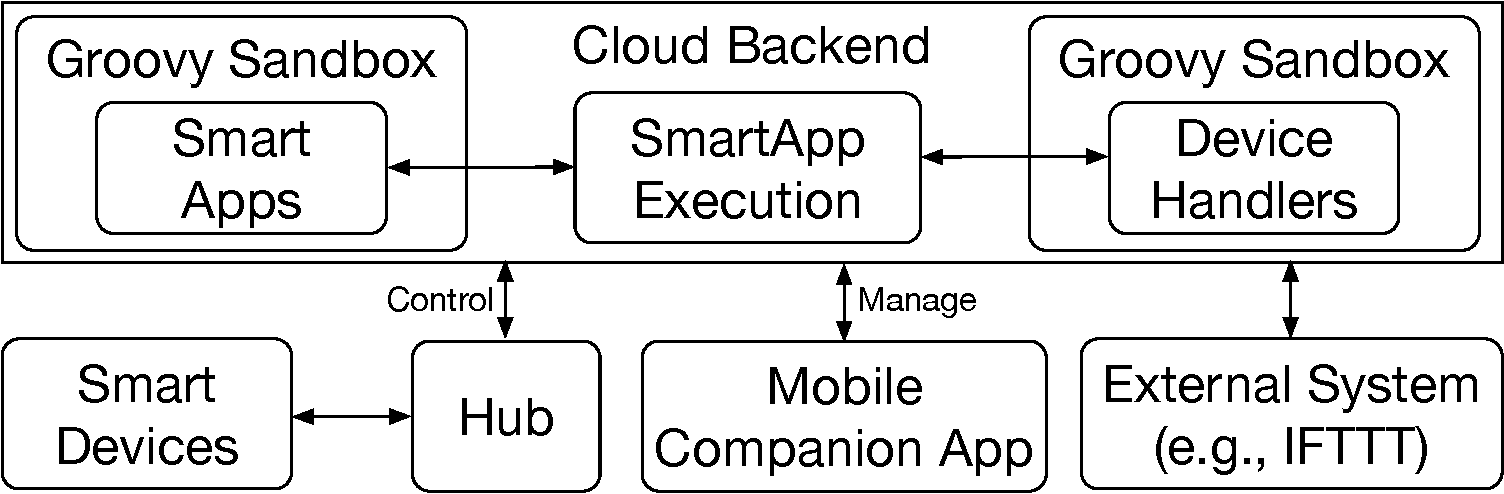
\includegraphics[width=3.0in]{SmartThingsArchitecture}
%\vspace{-0.1in}
\caption{SmartThings architecture overview.}
%\vspace{-.3in}
\label{SmartThingsArchitecture}
\end{center}
\end{figure}
%}
%\end{comment}

\subsection{Communications} {\color{black}ZigBee, which is build upon the PHY and MAC layers specified by IEEE 802.15.4, and Z-Wave, which adheres to the ITU-T G.9959 PHY and MAC layers, are among the most common wireless protocol stacks supported by an alliance of IoT product vendors \cite{Samsung:smartthingsproduct,Philips:hue,Yale:assurelock,Ecobee:thermostat}. Recent studies on link reliability of ZigBee and Z-Wave wireless networks have shown that one-hop retransmission is optionally supported by MAC layer and end-to-end retransmission is done by upper layers (\textit{e.g.}, application support sublayer) and depends on the implementation of the vendors \cite{s140814932,5747474,6379462,6392527,FULLER201744,7745306}.

Our study on communication protocols of Samsung SmartThings confirms that} the hub communicates with IoT devices using a protocol such as ZWave or ZigBee.
Experiments using the EZSync CC2531 Evaluation Module USB Dongle \cite{TI:CC2531} of
Texas Instruments, reveal that the ZigBee implementation
in SmartThings supports four (single hop) MAC layer retransmissions.
In addition, SmartThings has an application support sublayer that performs 15
end-to-end retransmissions (for a total of 60 retransmissions of a packet).
These are in line with ZigBee specifications as also verified in
\cite{s140814932,5747474,6379462,6392527}. Thus, typically,
it is rare that the system will transition to unsafe states because
of benign packet losses.


\begin{comment}
{
\thomas{ZigBee, which is build upon the PHY and MAC layers specified by IEEE 802.15.4, and Z-Wave, which adheres to the ITU-T G.9959 PHY and MAC layers, are among the most common wireless protocol stacks supported by an alliance of IoT product vendors \cite{Samsung:smartthingsproduct,Philips:hue,Yale:assurelock,Ecobee:thermostat}. Recent studies on link reliability of ZigBee and Z-Wave wireless networks have shown that one-hop retransmission is optionally supported by MAC layer and end-to-end retransmission is done by upper layers (\textit{e.g.}, application support sublayer) and depends on the implementation of the vendors \cite{s140814932,5747474,6379462,6392527,FULLER201744,7745306}. We have used the EZSync CC2531 Evaluation Module USB Dongle \cite{TI:CC2531} of Texas Instruments to evaluate the ZigBee communication protocols of Samsung SmartThings and found out that SmartThings' ZigBee supports four times of one-hop retransmissions and 15 times of end-to-end retransmissions. Therefore, we believe that SmartThings' ZigBee can guarantee end-to-end reliable transmission under normal conditions (\textit{e.g.}, without traffic jamming attacks) with the total number of 60 retransmissions.}
}
\end{comment}

\begin{comment}
{
\thomas{Many users have reported the failures of their ZigBee and Z-Wave IoT devices (\textit{e.g.}, motion sensors, water leak sensors, presence sensors, contact sensors, and garage door openers) in the SmartThings Community \cite{Samsung:smartthingscom1,Samsung:smartthingscom2, Samsung:smartthingscom3, Samsung:smartthingscom4}. Moreover, we have done some simple experiments to verify the behavior of the SmartThings system when device failure happens. The system under test comprises of a Samsung Hub, a Z-Wave smart lock, and a ZigBee smart power outlet. First, we unlocked the lock and turned on the outlet. As shown in the mobile companion app, the status of the lock was ``unlocked" and the status of the outlet was ``on". Second, we removed the battery of the lock and unpluged the outlet from the power strip. It took the mobile companion app about 12 minutes and 60 minutes to mark the outlet and the lock as ``unavailable'', but the status of the outlet was still ``on" and status of the lock was still ``unlocked". Even though the devices already stopped working, it took the SmartThings a long time to notify the failure to the users. During that time, an IoT system may enter bad states. Therefore, we need to take into account device failures when verifying IoT systems.}
}
\end{comment}

%\vspace{-.15in}
%\section{Misconfiguration Problems}
\section{Motivating Examples}
\label{sec:motivation}
{\color{black}We use two examples of violations found via our experiments (more details in \S~\ref{sec:eval}) to motivate our work.
Although simple, these examples exemplifies the safety problems that arise with third party IoT apps.

\subsection{Unsafe Physical States} In this example, a user installs three smart apps viz., \textit{Light Off When Close}, \textit{Good Night},
and \textit{Big Turn Off} to automate her smart home.
\textit{Light Off When Close} will turn off
configured lights when the configured contact sensor detects door closing;
\textit{Good Night} will change the location mode to \textit{Sleeping}
when all the monitored lights and motion sensors are inactive for
a configured period during night; and
\textit{Big Turn Off} will turn off all the configured devices
when (i) the user touches the app or (ii) the app detects a location mode change.

If we define a safety property as
\textit{temperature should always be higher than 0 degree Celsius},
a violation instance can be discovered by \sys as follows.
At night, after the owner closes the door monitored by
the \textit{Light Off When Close} app, it turns off the lights.
After a while, the app \textit{Good Night} changes the location mode to \textit{Sleeping}.
Upon the location mode change, \textit{Big Turn Off} turns off all of the configured devices,
which includes a heater.
Because the temperature can be below 0 degree during night,
this can lead to a violation of our safety property.

The violation scenario can be avoided if
(i) \textit{Big Turn Off} turns off the configured devices \emph{only} when the user touches the app,
(ii) \textit{Big Turn Off} explicitly asks users to configure that the configured devices to be turned off
only upon transitioning to a specific mode (\eg, ``Away''),
(iii) \textit{Big Turn Off} is installed together with only apps that change
the location mode to ``Away" when people leave home,
or (iv) \textit{Big Turn Off} is not configured to the heater.
Unfortunately, the first three options are not feasible and users may
have valid reasons to configure the app to control the heater.}

\subsection{Misconfiguration Problems} Besides malicious apps, misconfiguration is a common cause for safety violations.
When installing a smart app, a user has
to configure the app with sensor(s) and actuator(s). Poor configurations
can transition the IoT system to unsafe physical states.
There are many common causes for such misconfigurations, \eg,
(i) the app's description is unclear,
(ii) there are too many configuration options,
and (iii) normal users often do not have good domain knowledge to
clearly understand the behaviors of smart devices and smart apps.
To exemplify these issues, we conduct a user study (more details in \S\ref{sec:eval})
where we asked 7 student volunteers to configure various apps as they deemed fit.
Among these apps, one app is called \textit{Virtual Thermostat} and describes itself as
``Control a space heater or window air conditioner (AC) in conjunction with any temperature sensor, like a SmartSense Multi.''
{\color{black}Figure~\ref{inputexample} shows the inputs needed from a user,
which include a temperature measurement sensor (lines 2-4),
the power outlets into which the heater or the AC are plugged (lines 5-7),
a desired temperature (lines 8-10), etc.}
Although the developers use the word {\em or} and the app only expects
either a heater or an AC,
5 out of 7 student volunteers thought the app controls {\em both}
a heater and an AC to maintain the desired temperature and
mis-configured the app to control both the AC outlet and the heater outlet.
To exacerbate the confusion, the app expects
the configuration of outlets (\texttt{capability.switch})
instead of the actual devices that are plugged into the outlets
(\ie, AC or heater) (note that the SmartThings UI displays all available outlets to the user).
As a result of volunteer misconfigurations, when the temperature is higher than a predefined threshold,
the \textit{Virtual Thermostat} would turn on both the configured outlets
(\ie, both the heater and the AC).
This violates the following two commonsense properties:
(i) a heater is turned on when temperature is above a predefined threshold and
(ii) an AC and a heater are both turned on.

\begin{figure}[tb]
%\scriptsize
%\tiny
\begin{center}
\ssp
\lstinputlisting[language=groovy]{./code/virtualthermostat.groovy}
%\vspace{-0.17in}
\caption{{\color{black}Example of input info needed from users to configure the app \textit{Virtual Thermostat}.}}
\label{inputexample}
\end{center}
%\vspace{-0.22in}
\end{figure}

{\color{black}While these examples are quite simple, it exemplifies an important problem:
it is very possible that users may not carefully evaluate their IoT systems so
it can be driven into bad states,
especially when apps are installed or configured at different times
or by different users.
In practice, it is also difficult for typical users who do not have a strong
technical background to assess if bad interactions are possible.
Even if cursory examinations reveal simple violations,
complex violations are harder to find manually.
The latter is true especially if such interactions result from a chain of
sensing and actuation events across multiple devices controlled
by independent apps.
Thus, an automated way of discovering such bad interactions is necessary.}

\begin{comment}
\begin{figure}[tb]
\begin{center}
\includegraphics[width=3.0in]{inputexample}
%\vspace{-0.1in}
\caption{{\color{black}Example of input info needed from users to configure the app \textit{Virtual Thermostat}.}}
\label{inputexample}
\end{center}
%\vspace{-0.25in}
\end{figure}
\end{comment}


%\vspace{-0.14in}
\section{Model Checking as a Building Block}
The problem of reasoning if and why the IoT system
could transition into a bad physical state
is challenging because the number of apps and devices is likely to
grow in the future and thus, analyzing all possible interactions
between them will be hard.
Static analysis tools tend to sacrifice completeness for soundness,
and thus result in lots of false positives.
In contrast, typical dynamic analyses tools
verify the properties of a program during execution,
but can lead to false negatives.

Model checking is a technique that checks
whether a system meets a given specification~\cite{jhala2009software},
%In software model checking~\cite{jhala2009software},
%the system is a program and specifications are safety and liveness properties.
by systematically exploring the program's state.
In an ideal case, the model checker exhaustively examines all possible system states to verify
{\color{black}if there is any violation} of specifications relating
to safety and/or liveness properties.
%However, the undecidability of the halting problem implies that for
%complex systems such as IoT, neither 
%general analysis algorithm that can be both sound and complete.
\textcolor{black}{However, the complexity of modern system software makes this extremely challenging computationally.}
So in practice, when the goal is to find bugs, a model checker is usually
used as a \emph{falsifier} \ie, it explores a portion of the reachable state
space and tries to find a computation that violates the specified property.
This is sometimes
also called bounded model checking~\cite{Biere1999:BMC, Kroening2014:CBMC, Merz2012:LLBMC, Cordeiro2012:ESBMC,Roya:networkprotocol}.

We adopt model checking as a basic building block since:
(i) it provides the flexibility towards verifying
all the desired properties with linear temporal logic\footnote{
  Linear temporal logic (LTL) is
  a modal temporal logic with modalities referring to time.
  LTL is used to verify
  properties of reactive systems~\cite{Baier:modelchecking}.},
(ii) it provides concrete counter-examples~\cite{Baier:modelchecking,Spin:intro}
which are very useful in analyzing why and how the bad states occur,
(iii) its holistic nature of checking can capture interactions among multiple apps,
and (iv) it is more efficient than exhaustive testing \cite{10.1007/978-3-319-70389-3_7}.
%
However, a successful model checker must address the state explosion problem,
\ie, the state space could become unwieldy and requires exponential time to explore.

%\begin{comment}
{\color{black}Model checking can be grouped into two classes:
(a) explicit model checking~\cite{Clarke1982} where progress is made one state at a time and,
(b) symbolic model checking~\cite{McMillan1993} that examines sets of states in each step.
Literature suggests that neither is a clear winner 
with regards to yielding complete verification within reasonable times
in all settings~\cite{Avrunin2000:benchmarking,Eisner2002:comparing,Holzmann1999:iprotocol}.

In brief, symbolic model checking is considered to perform better for synchronous hardware systems
and explicit model checking is better for concurrent software systems
\cite{Flavio2003:symbolicmodelchecking,Choi2007:nusmvtospin,Dong1999:fighting}.
Biere~\etal, claim that explicit model checking is the most efficient model checking technique in practice
if the number of reachable states is small, \ie,
below several million states~\cite{Armin2001:verifyingsequentialbehavior}.
Eisner~\etal argue that a symbolic model checker performs better even for
asynchronous systems~\cite{Eisner2002:comparing}.
However, there are other reports that indicate that a
direct comparison of the two categories is almost impossible
\cite{Avrunin2000:benchmarking,Eisner2002:comparing,Holzmann1999:iprotocol}.}
%
%}
%\end{comment}

{\color{black}Given its popularity and flexibility in modelling both concurrent and synchronous systems \cite{Flavio2003:symbolicmodelchecking,Choi2007:nusmvtospin,Dong1999:fighting}, we use \spin~\cite{Holzmann:spin} for checking if a given set of safety properties can be possibly violated.}
%Specifically, we use the popular \spin model checker~\cite{Holzmann:spin} for
%checking if a given set of safety properties can be possibly violated.
%\spin is a popular open-source software model checking tool,
%used for the formal verification of multi-threaded software applications.
Since an IoT system may be composed of a large number of apps and smart devices,
we use \spin's verification mode with BITSTATE hashing---an approximate technique
that stores the hash code of states in a bitfield instead of storing the whole states.
Although the BITSTATE hashing technique does not provide a complete verification,
empirical results and theoretical analysis have proved its effectiveness
in terms of state coverage
\cite{Holzmann1998,Cattel94,Chaves91,Holzmann94:NewCoRe,Holzmann94:prove}.
